\subsection*{The Graph of a Real Function}
We will finish this section with methods to visually communicate information about two specific types of functions.  The first is the familiar method of graphing functions that was a major part of some previous mathematics courses.  For example, consider the function $g \x \R \to \R$ defined by $g(x) = x^2 - 2x - 1$.

\begin{figure}[h]
\begin{center}
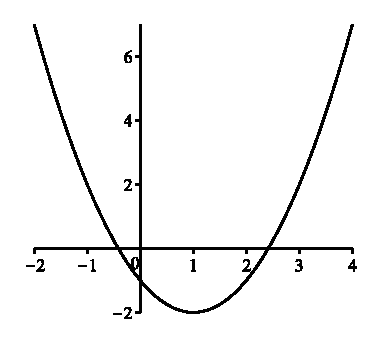
\includegraphics{figps-graphsec6-1.eps} 
\caption{Graph of $y = g( x )$, where  $g( x ) = x^2  - 2x - 1$} \label{fig:functiongraph1}
\end{center}
\end{figure}
Every point on this graph corresponds to an ordered pair  $\left( {x,\;y} \right)$ of real numbers, where  $y = g( x ) = x^2  - 2x - 1$.  Because we use the Cartesian plane when drawing this type of graph, we can only use this type of graph when both the domain and the codomain of the function are subsets of the real numbers  
$\R$.  Such a function is sometimes called a \textbf{real function}.
\label{realfunction}%
\index{real function}%
\index{function!real}%
 The graph of a real function is a visual way to communicate information about the function.  For example, the range of $g$ is the set of all  $y$-values  that correspond to points on the graph.  In this case, the graph of $g$ is a parabola and has a vertex at the point $(1, -2)$.  (\note The $x$-coordinate of the vertex can be found by using calculus and solving the equation $f ' (x) = 0$.)  Since the graph of the function $g$ is a parabola, we know that the pattern shown on the left end and the right end of the graph continues and we can conclude that the range of $g$ is the set of all $y \in \R$ such that $y \geq -2$.  That is,
\[
\text{range} (g) = \{ y \in \R \mid y \geq -2 \}.
\]
\hbreak

\begin{prog}[\textbf{Using the Graph of a Real Function}] \label{pr:graphreal} \hfill \\ 
The graph in Figure~\ref{fig:functiongraph2} shows the graph of (slightly more than) two complete periods for a function $f \x \R \to \R$, where $f(x) = A \sin (Bx)$ for some positive real number constants $A$ and $B$.
\begin{figure}[h]
\begin{center}
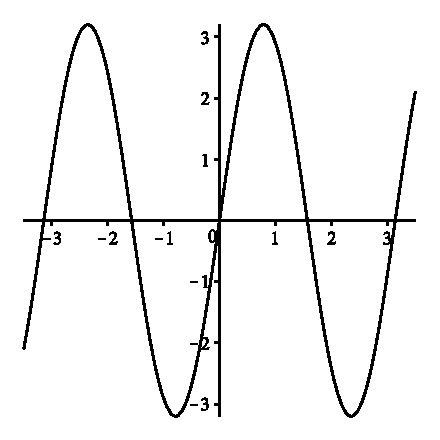
\includegraphics{figps-graph2sec6-1.eps} 
\caption{Graph of $y = f( x )$} \label{fig:functiongraph2}
\end{center}
\end{figure}
\begin{enumerate}
  \item We can use the graph to estimate the output for various inputs.  This is done by estimating the $y$-coordinate for the point on the graph with a specified $x$-coordinate.  On the graph, draw vertical lines at  $x =  - 1$  and  $x = 2$ and estimate the values of  $f( { - 1} )$  and  $f( 2 )$.
  \item Similarly, we can estimate inputs of the function that produce a specified output.  This is done by estimating the $x$-coordinates of the points on the graph that have a specified 
$y$-coordinate.  Draw a horizontal line at  $y = 2$ and estimate at least two values of  $x$  such that  
$f( x ) = 2$.
  \item Use the graph in Figure~\ref{fig:functiongraph2} to estimate the range of the function $f$.
\end{enumerate}
\end{prog}
\hbreak


\endinput

